%& -shell-escape
\documentclass[a4paper,12pt]{article}
\usepackage[legalpaper, portrait , margin=1.5cm]{geometry}
\usepackage[latin1]{inputenc}
\usepackage[T1]{fontenc}
\usepackage[italian]{babel}
\usepackage{wrapfig}
\usepackage{graphicx}
\graphicspath{ {./Sorgenti/} }
\usepackage{enumitem}
\usepackage{pifont}

\author{Alfano Emanuele \\ Badalamenti Filippo \\ Vitti Gabriele}

\begin{document}
\title{Cinematiche Dirette Robot}
\maketitle
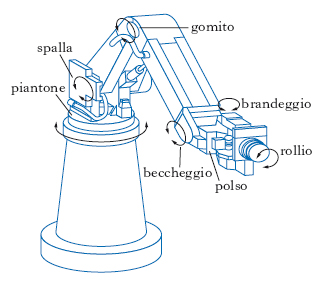
\includegraphics[width=\textwidth]{scorbot.jpg}
\pagebreak

\section*{Metodo di Denavit Hartenberg}

	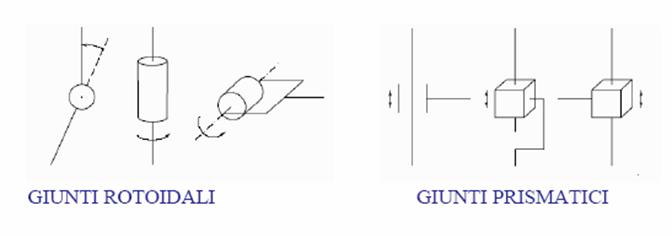
\includegraphics[width=\textwidth]{tipiGiunti.jpg}

Il metodo di D-H standardizza un metodo per ottenere la cinematica diretta di un qualunque robot 3D.

Conoscendo uno schema dei giunti di un robot, tutti presi a 1 DOF (Degree of Freedom) � possibile ricostruire qualsiasi struttura.

Posizionando i vari sistemi di riferimento con la procedura di D-H � possibile automatizzare il processo di ottenimento della cinematica diretta.
Considerando due [[giunto (meccanica)|giunti]] consecutivi:


\begin{itemize}


	\item L'asse $Z_{i-1}$ si sceglie coincidente con l'asse del giunto $i$, l'asse $Z_i$ coincidente con l'asse del giunto $i+1$;
	
	\item L'asse $X_{i}$ deve essere scelto in base a come si posizionano tra di loro gli assi $i$ e $i-1$:
	
	
	
	\begin{minipage}{0.4\textwidth}
		\begin{itemize}[label=\ding{212}]
			\item Se $Z_{i} \cong Z_{i-1}$  allora $\longrightarrow X_{i}=~Z_{i-1}\perp Z_{i}$ e orientamento a piacere.
			
			\item Se $Z_{i} \parallel Z_{i-1}$ ma non sovrapposto $\longrightarrow X_{i}=~Z_{i-1}\perp Z_{i}$ dove in questo caso
			 � la prosecuzione di uno dei segmenti di minima distanza.
			
			\item Se $Z_{i}$ coincide in un punto soltanto con $Z_{i-1}$, quello sar� $O_{i} \longrightarrow X_{i}=~Z_{i-1}\perp Z_{i}$ 
			
			\item Se $Z_{i}$ � sghemba con $Z_{i-1}$, $O_{i}$ � preso lungo il segmento di minima distanza che li unisce e $X_{i}$ si
			trova lungo questo asse 
		\end{itemize}
	\end{minipage}
	\hfill % dice al compilatore di non andare a capo ma di mettere tanti spazi quanto necessario per far toccare il successivo blocco a destra, il compilatore potrebbe mettere anche 0 e quello che c'� dopo finisce fuori pagina, ma cmq non va a capo
	\begin{minipage}{0.52\textwidth}% adapt widths of minipages to your needs
			\centering{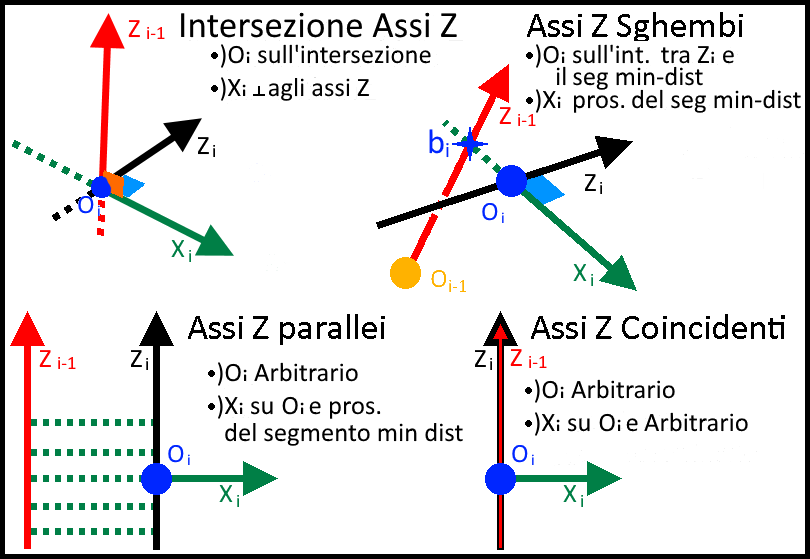
\includegraphics[width=\textwidth]{deanavit-hattemberg.png}}
	\end{minipage}%
		
	\item I restanti assi $Y_{n-1}$ e $Y_n$ sono scelti in modo da completare le rispettive terne affinch� diventino destre.
\end{itemize}

\begin{minipage}{0.7\textwidth}
 Una volta fatto ci� bisogna risalire i sistemi di riferimento portando a far coincidere il sistema $R_{i-1}$ con il sistema $R_{i}$
 muovendo nell'ordine le variabili: $\theta, d ,\alpha, a$ e salvando nella tabella i valori:
 
 A questo punto baster� montare tra di loro le varie matrici di avvitamento ottenendo la matrice della cinematica diretta:
\end{minipage}
\hfill
\begin{minipage}{0.3\textwidth}
\begin{tabular}{p{0.5cm}|p{0.5cm}|p{0.5cm}|p{0.5cm}|p{0.5cm}|}
		\cline{2-5} &
		\multicolumn{2}{|c|}{$A_z(\theta,d)$} &
		\multicolumn{2}{|c|}{$A_x(\alpha,a)$} \\
		\hline
		\multicolumn{1}{|c|}{$R_1$} &  &  &  &  \\
		\hline
		\multicolumn{1}{|c|}{$R_{...}$} &  &  &  &  \\
		\hline
		\multicolumn{1}{|c|}{$R_n$} &  &  &  &  \\
		\hline
\end{tabular}
\end{minipage}

\large $Q_{0,n}=A_z(\theta,d)_{R_1} \cdot A_x(\alpha,a)_{R_1} \cdot A_z(\theta,d)_{R_2} \cdot A_x(\alpha,a)_{R_2} \cdot ... \cdot A_z(\theta,d)_{R_n} \cdot A_x(\alpha,a)_{R_n}$
	


\section*{Cartesiano}
\begin{minipage}{0.5\textwidth}
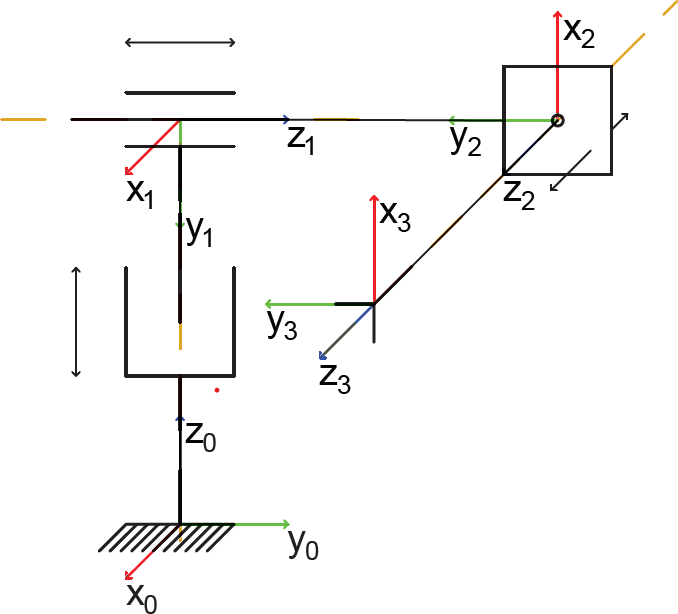
\includegraphics[width=\textwidth]{Strutture/Cartesiano.png}
\end{minipage}
\hfill
\begin{minipage}{0.5\textwidth}
\centering
\begin{tabular}{c|c|c|c|c|}
            \cline{2-5} &
            \multicolumn{2}{|c|}{$A_z(\theta,d)$} &
            \multicolumn{2}{|c|}{$A_x(\alpha,a)$} \\
            \hline
        \multicolumn{1}{|c|}{$R_1$} & $0$ & $q_{1}$ & $-{{\pi}\over{2}}$ & $0$ \\
            \hline
        \multicolumn{1}{|c|}{$R_2$} & $-{{\pi}\over{2}}$ & $q_{2}$ & $-{{\pi}\over{2}}$ & $0$ \\
            \hline
        \multicolumn{1}{|c|}{$R_3$} & $0$ & $q_{3}$ & $0$ & $0$ \\
            \hline
\end{tabular}

$$\ifx\endpmatrix\undefined\pmatrix{\else\begin{pmatrix}\fi 0&0&1&
 q_{3}\cr 0&-1&0&q_{2}\cr 1&0&0&q_{1}\cr 0&0&0&1\cr 
 \ifx\endpmatrix\undefined}\else\end{pmatrix}\fi $$

\end{minipage}


\section*{Cilindrico}
\begin{minipage}{0.5\textwidth}
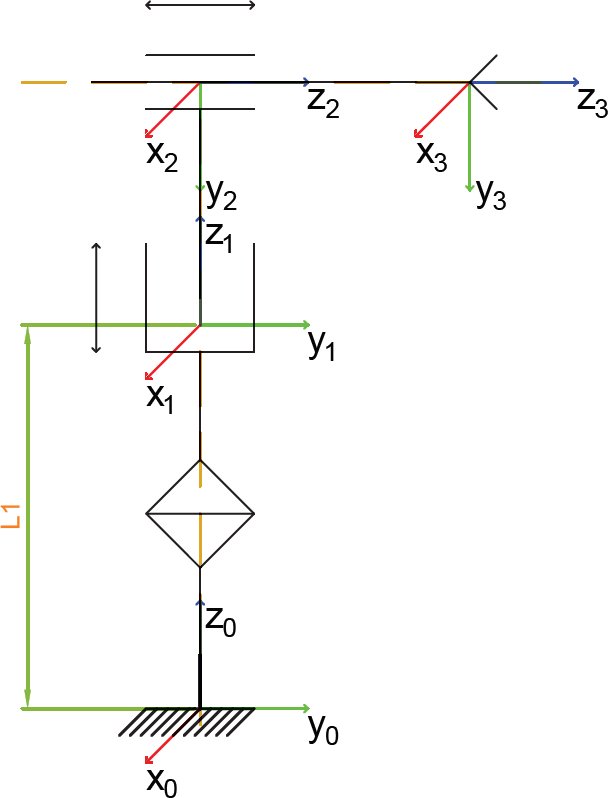
\includegraphics[width=\textwidth]{Strutture/Cilindrico.png}
\end{minipage}
\hfill
\begin{minipage}{0.5\textwidth}
\centering
\begin{tabular}{c|c|c|c|c|}
            \cline{2-5} &
            \multicolumn{2}{|c|}{$A_z(\theta,d)$} &
            \multicolumn{2}{|c|}{$A_x(\alpha,a)$} \\
            \hline
        \multicolumn{1}{|c|}{$R_1$} & $q_{1}$ & $0$ & $0$ & $D_{1}$ \\
            \hline
        \multicolumn{1}{|c|}{$R_2$} & $q_{2}$ & $0$ & $0$ & $D_{2}$ \\
            \hline
        \multicolumn{1}{|c|}{$R_3$} & $q_{3}$ & $0$ & $0$ & $D_{3}$ \\
            \hline
\end{tabular}

$$\ifx\endpmatrix\undefined\pmatrix{\else\begin{pmatrix}\fi \cos 
 q_{1}&0&-\sin q_{1}&-\sin q_{1}\,q_{3}\cr \sin q_{1}&0&\cos q_{1}&
 \cos q_{1}\,q_{3}\cr 0&-1&0&q_{2}+L_{1}\cr 0&0&0&1\cr 
 \ifx\endpmatrix\undefined}\else\end{pmatrix}\fi $$

\end{minipage}


\section*{RRR Planare}

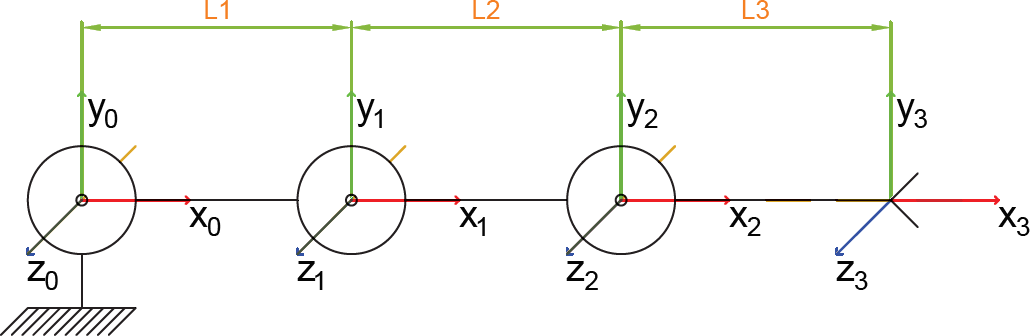
\includegraphics[width=\textwidth]{Strutture/RRRplanare.png}
\centering
\begin{tabular}{c|c|c|c|c|}  
            \cline{2-5} &
            \multicolumn{2}{|c|}{$A_z(\theta,d)$} &
            \multicolumn{2}{|c|}{$A_x(\alpha,a)$} \\
            \hline
        \multicolumn{1}{|c|}{$R_1$} & $q_{1}$ & $0$ & $0$ & $D_{1}$ \\
            \hline
        \multicolumn{1}{|c|}{$R_2$} & $q_{2}$ & $0$ & $0$ & $D_{2}$ \\
            \hline
        \multicolumn{1}{|c|}{$R_3$} & $q_{3}$ & $0$ & $0$ & $D_{3}$ \\
            \hline
\end{tabular}

\scriptsize{$$\pmatrix{-\left(\cos q_{1}\,\sin q_{2}\,\sin q_{3}+\sin q_{1}\,
 \cos q_{2}\,\sin q_{3}+\sin q_{1}\,\sin q_{2}\,\cos q_{3}-\cos q_{1}
 \,\cos q_{2}\,\cos q_{3}\right)&\sin q_{1}\,\sin q_{2}\,\sin q_{3}-
 \cos q_{1}\,\cos q_{2}\,\sin q_{3}-\cos q_{1}\,\sin q_{2}\,\cos 
 q_{3}-\sin q_{1}\,\cos q_{2}\,\cos q_{3}&0\cr -\left(\sin q_{1}\,\sin q_{2}
 \,\sin q_{3}-\cos q_{1}\,\cos q_{2}\,\sin q_{3}-\cos q_{1}\,\sin 
 q_{2}\,\cos q_{3}-\sin q_{1}\,\cos q_{2}\,\cos q_{3}\right)&-\left(
 \cos q_{1}\,\sin q_{2}\,\sin q_{3}+\sin q_{1}\,\cos q_{2}\,\sin 
 q_{3}+\sin q_{1}\,\sin q_{2}\,\cos q_{3}-\cos q_{1}\,\cos q_{2}\,
 \cos q_{3}\right)&0\cr 0&0&1\cr 0&0&0\cr }$$

$$\pmatrix{0&-\left(D_{3}\,\cos q_{1}
 \,\sin q_{2}\,\sin q_{3}+D_{3}\,\sin q_{1}\,\cos q_{2}\,\sin q_{3}+
 D_{3}\,\sin q_{1}\,\sin q_{2}\,\cos q_{3}-D_{3}\,\cos q_{1}\,\cos 
 q_{2}\,\cos q_{3}+D_{2}\,\sin q_{1}\,\sin q_{2}-D_{2}\,\cos q_{1}\,
 \cos q_{2}-D_{1}\,\cos q_{1}\right)\cr0&-\left(D_{3}\,\sin q_{1}\,\sin q_{2}\,\sin q_{3}
 -D_{3}\,\cos q_{1}\,\cos q_{2}\,\sin q_{3}-D_{3}\,\cos q_{1}\,\sin 
 q_{2}\,\cos q_{3}-D_{3}\,\sin q_{1}\,\cos q_{2}\,\cos q_{3}-D_{2}\,
 \cos q_{1}\,\sin q_{2}-D_{2}\,\sin q_{1}\,\cos q_{2}-D_{1}\,\sin 
 q_{1}\right)\cr 1&0\cr 0&1\cr }$$


$$\pmatrix{-\left(\cos q_{1}\,\sin q_{2}\,\sin q_{3}+\sin q_{1}\,
 \cos q_{2}\,\sin q_{3}+\sin q_{1}\,\sin q_{2}\,\cos q_{3}-\cos q_{1}
 \,\cos q_{2}\,\cos q_{3}\right)&\sin q_{1}\,\sin q_{2}\,\sin q_{3}-
 \cos q_{1}\,\cos q_{2}\,\sin q_{3}-\cos q_{1}\,\sin q_{2}\,\cos 
 q_{3}-\sin q_{1}\,\cos q_{2}\,\cos q_{3}&0\cr -\left(\sin q_{1}\,\sin q_{2}
 \,\sin q_{3}-\cos q_{1}\,\cos q_{2}\,\sin q_{3}-\cos q_{1}\,\sin 
 q_{2}\,\cos q_{3}-\sin q_{1}\,\cos q_{2}\,\cos q_{3}\right)&-\left(
 \cos q_{1}\,\sin q_{2}\,\sin q_{3}+\sin q_{1}\,\cos q_{2}\,\sin 
 q_{3}+\sin q_{1}\,\sin q_{2}\,\cos q_{3}-\cos q_{1}\,\cos q_{2}\,
 \cos q_{3}\right)&0\cr 0&0&1\cr 0&0&0\cr }$$

$$\left.\begin{array}{cc}
0&-\left(D_{3}\,\cos q_{1}
 \,\sin q_{2}\,\sin q_{3}+D_{3}\,\sin q_{1}\,\cos q_{2}\,\sin q_{3}+
 D_{3}\,\sin q_{1}\,\sin q_{2}\,\cos q_{3}-D_{3}\,\cos q_{1}\,\cos 
 q_{2}\,\cos q_{3}+D_{2}\,\sin q_{1}\,\sin q_{2}-D_{2}\,\cos q_{1}\,
 \cos q_{2}-D_{1}\,\cos q_{1}\right)\\0&-\left(D_{3}\,\sin q_{1}\,\sin q_{2}\,\sin q_{3}
 -D_{3}\,\cos q_{1}\,\cos q_{2}\,\sin q_{3}-D_{3}\,\cos q_{1}\,\sin 
 q_{2}\,\cos q_{3}-D_{3}\,\sin q_{1}\,\cos q_{2}\,\cos q_{3}-D_{2}\,
 \cos q_{1}\,\sin q_{2}-D_{2}\,\sin q_{1}\,\cos q_{2}-D_{1}\,\sin 
 q_{1}\right)\\ 1&0\\ 0&1\\ \end{array}\right)$$
}



\section*{Sferico 1}
\begin{minipage}{0.35\textwidth}
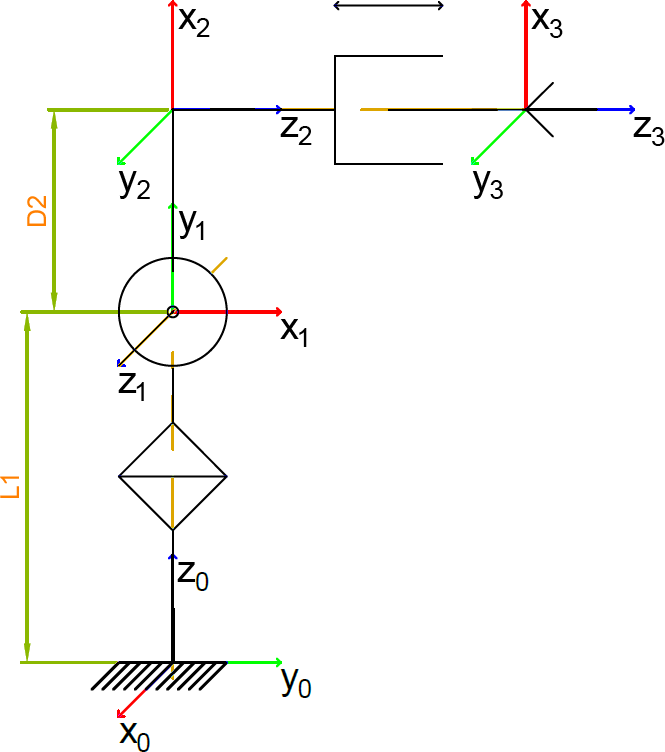
\includegraphics[width=\textwidth]{Strutture/Sferico1.png}
\end{minipage}
\hfill
\begin{minipage}{0.65\textwidth}
\centering
\begin{tabular}{c|c|c|c|c|}
            \cline{2-5} &
            \multicolumn{2}{|c|}{$A_z(\theta,d)$} &
            \multicolumn{2}{|c|}{$A_x(\alpha,a)$} \\
            \hline
        \multicolumn{1}{|c|}{$R_1$} & $q_{1}$ & $0$ & $0$ & $D_{1}$ \\
            \hline
        \multicolumn{1}{|c|}{$R_2$} & $q_{2}$ & $0$ & $0$ & $D_{2}$ \\
            \hline
        \multicolumn{1}{|c|}{$R_3$} & $q_{3}$ & $0$ & $0$ & $D_{3}$ \\
            \hline
\end{tabular}

\end{minipage}


\section*{Sferico di Stanford}
\begin{minipage}{0.5\textwidth}
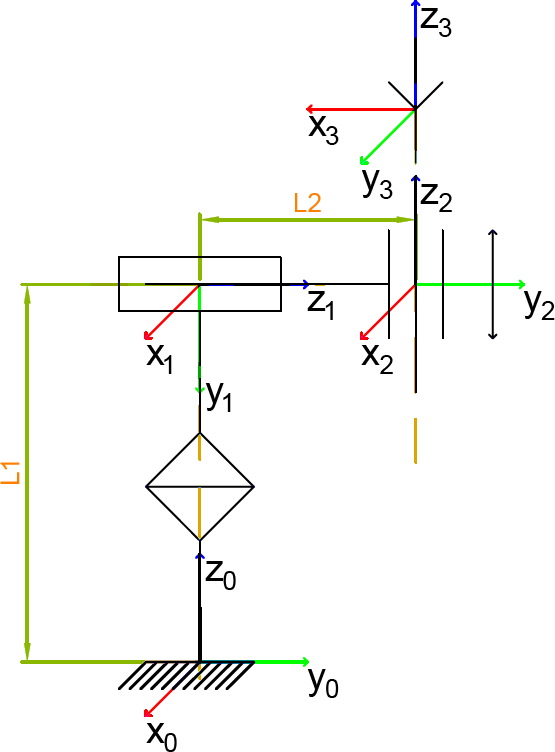
\includegraphics[width=\textwidth]{Strutture/SfericoStanford.png}
\end{minipage}
\hfill
\begin{minipage}{0.5\textwidth}
\centering
\begin{tabular}{c|c|c|c|c|}
            \cline{2-5} &
            \multicolumn{2}{|c|}{$A_z(\theta,d)$} &
            \multicolumn{2}{|c|}{$A_x(\alpha,a)$} \\
            \hline
        \multicolumn{1}{|c|}{$R_1$} & $q_{1}$ & $0$ & $0$ & $D_{1}$ \\
            \hline
        \multicolumn{1}{|c|}{$R_2$} & $q_{2}$ & $0$ & $0$ & $D_{2}$ \\
            \hline
        \multicolumn{1}{|c|}{$R_3$} & $q_{3}$ & $0$ & $0$ & $D_{3}$ \\
            \hline
\end{tabular}

\end{minipage}


\section*{Antropomorfo}
\begin{minipage}{0.5\textwidth}
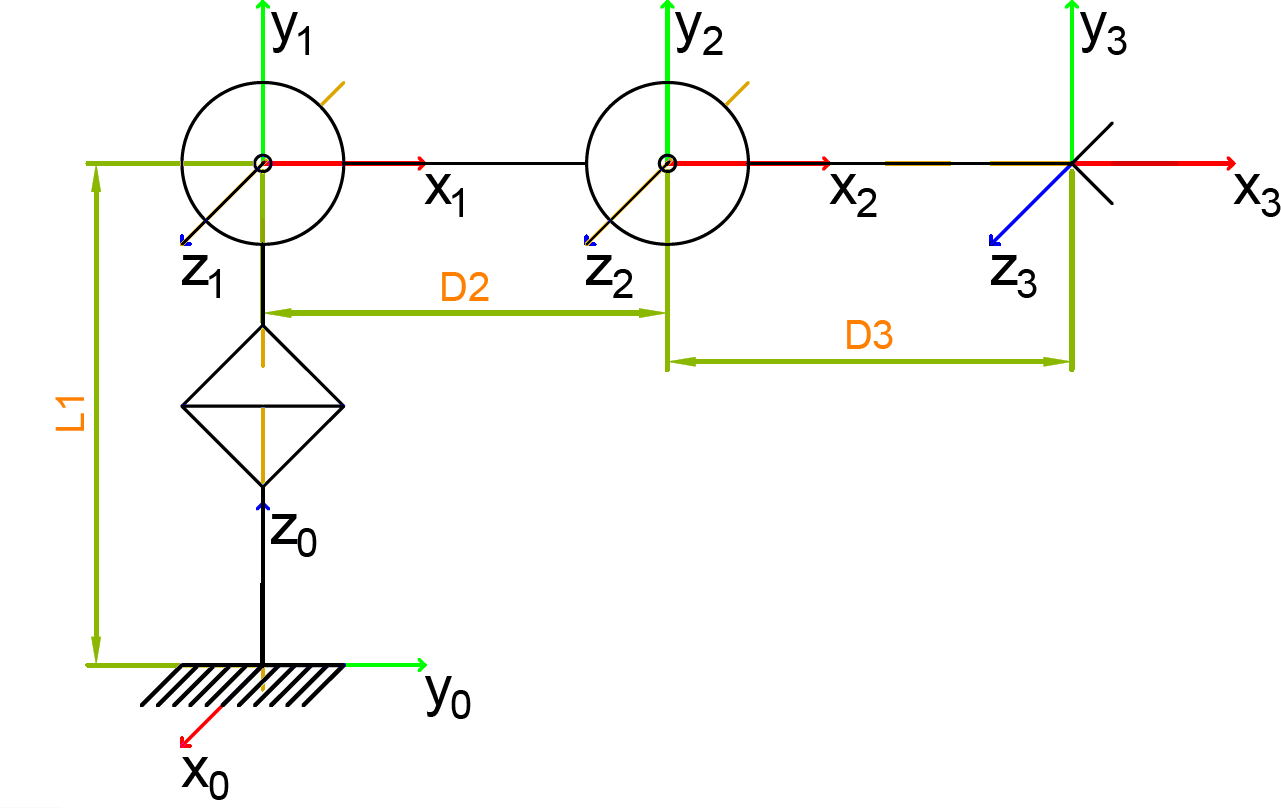
\includegraphics[width=\textwidth]{Strutture/Antropomorfo.png}
\end{minipage}
\hfill
\begin{minipage}{0.5\textwidth}
\centering
\begin{tabular}{c|c|c|c|c|}
            \cline{2-5} &
            \multicolumn{2}{|c|}{$A_z(\theta,d)$} &
            \multicolumn{2}{|c|}{$A_x(\alpha,a)$} \\
            \hline
        \multicolumn{1}{|c|}{$R_1$} & $q_{1}$ & $0$ & $0$ & $D_{1}$ \\
            \hline
        \multicolumn{1}{|c|}{$R_2$} & $q_{2}$ & $0$ & $0$ & $D_{2}$ \\
            \hline
        \multicolumn{1}{|c|}{$R_3$} & $q_{3}$ & $0$ & $0$ & $D_{3}$ \\
            \hline
\end{tabular}

\end{minipage}


\section*{Polso Sferico}
\begin{minipage}{0.5\textwidth}
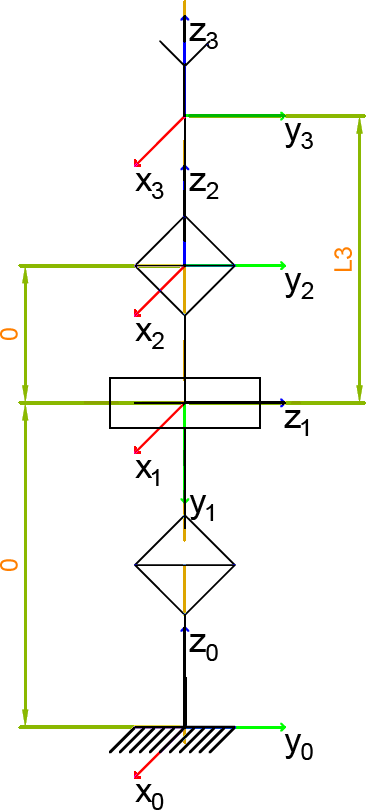
\includegraphics[width=\textwidth]{Strutture/PolsoSferico.png}
\end{minipage}
\hfill
\begin{minipage}{0.5\textwidth}
\centering
\begin{tabular}{c|c|c|c|c|}
            \cline{2-5} &
            \multicolumn{2}{|c|}{$A_z(\theta,d)$} &
            \multicolumn{2}{|c|}{$A_x(\alpha,a)$} \\
            \hline
        \multicolumn{1}{|c|}{$R_1$} & $q_{1}$ & $0$ & $0$ & $D_{1}$ \\
            \hline
        \multicolumn{1}{|c|}{$R_2$} & $q_{2}$ & $0$ & $0$ & $D_{2}$ \\
            \hline
        \multicolumn{1}{|c|}{$R_3$} & $q_{3}$ & $0$ & $0$ & $D_{3}$ \\
            \hline
\end{tabular}

\end{minipage}


\section*{Cartesiano con Polso}
\begin{minipage}{0.5\textwidth}
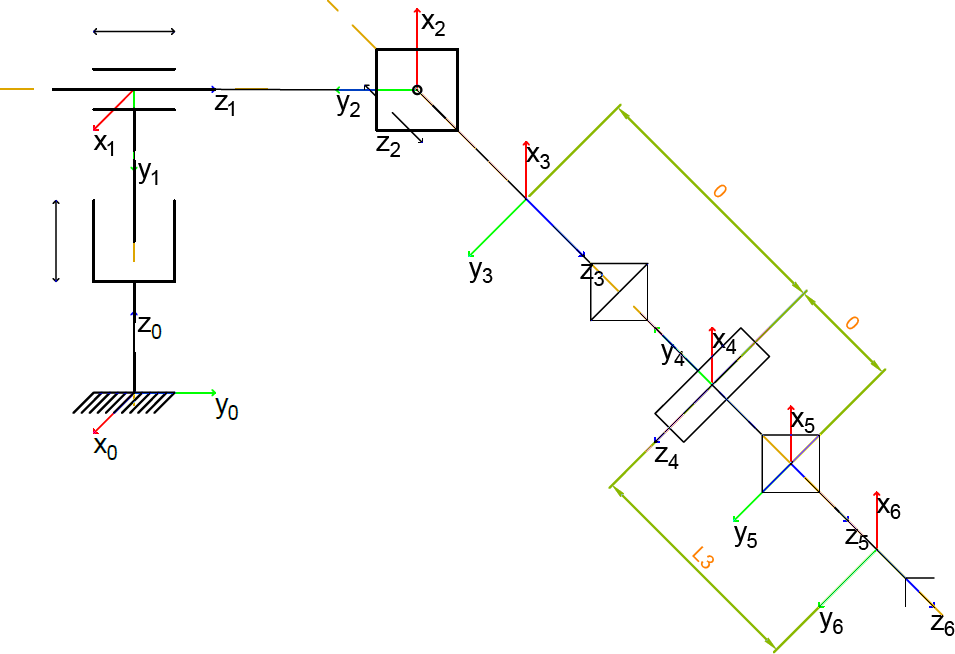
\includegraphics[width=\textwidth]{Strutture+Polso/Cartesiano+p.png}
\end{minipage}
\hfill
\begin{minipage}{0.5\textwidth}
\centering
\begin{tabular}{c|c|c|c|c|}
            \cline{2-5} &
            \multicolumn{2}{|c|}{$A_z(\theta,d)$} &
            \multicolumn{2}{|c|}{$A_x(\alpha,a)$} \\
            \hline
        \multicolumn{1}{|c|}{$R_1$} & $q_{1}$ & $0$ & $0$ & $D_{1}$ \\
            \hline
        \multicolumn{1}{|c|}{$R_2$} & $q_{2}$ & $0$ & $0$ & $D_{2}$ \\
            \hline
        \multicolumn{1}{|c|}{$R_3$} & $q_{3}$ & $0$ & $0$ & $D_{3}$ \\
            \hline
\end{tabular}

\end{minipage}


\section*{Cilindrico con Polso}
\begin{minipage}{0.5\textwidth}
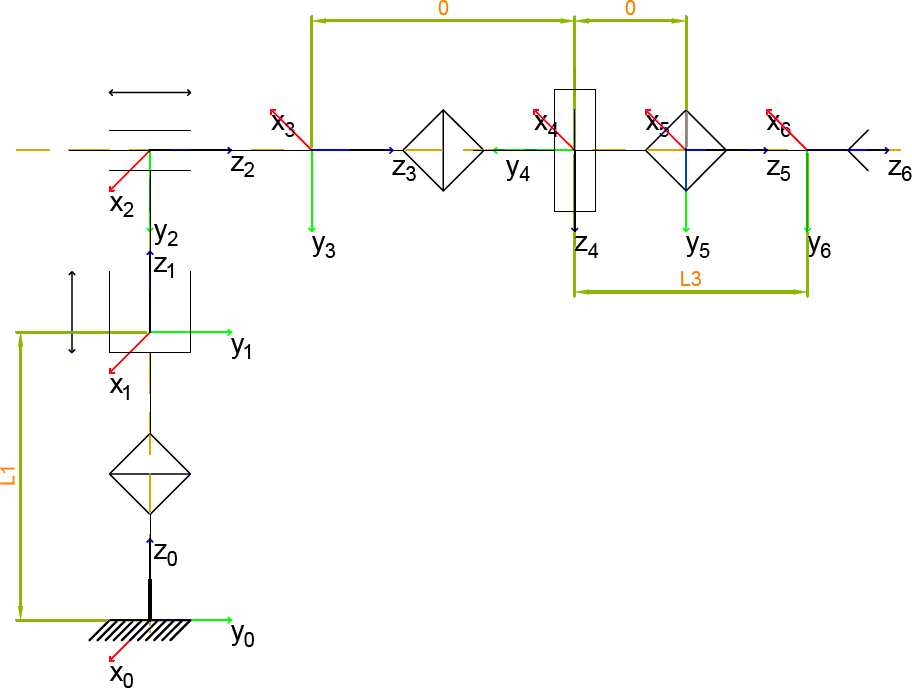
\includegraphics[width=\textwidth]{Strutture+Polso/Cilindrico+p.png}
\end{minipage}
\hfill
\begin{minipage}{0.5\textwidth}
\centering
\begin{tabular}{c|c|c|c|c|}  
            \cline{2-5} &
            \multicolumn{2}{|c|}{$A_z(\theta,d)$} &
            \multicolumn{2}{|c|}{$A_x(\alpha,a)$} \\
            \hline
        \multicolumn{1}{|c|}{$R_1$} & $q_{1}$ & $L_{1}$ & $0$ & $0$ \\
            \hline
        \multicolumn{1}{|c|}{$R_2$} & $0$ & $q_{2}$ & $-{{\pi}\over{2}}$ & $0$ \\
            \hline
        \multicolumn{1}{|c|}{$R_3$} & $0$ & $q_{3}$ & $0$ & $0$ \\
            \hline
        \multicolumn{1}{|c|}{$R_4$} & $q_{4}$ & $0$ & $-{{\pi}\over{2}}$ & $0$ \\
            \hline
        \multicolumn{1}{|c|}{$R_5$} & $q_{5}$ & $0$ & ${{\pi}\over{2}}$ & $0$ \\
            \hline
        \multicolumn{1}{|c|}{$R_6$} & $q_{6}$ & $L_{6}$ & $0$ & $0$ \\
            \hline
\end{tabular}

\end{minipage}


\section*{RRR Planare con Polso}
\begin{minipage}{0.5\textwidth}
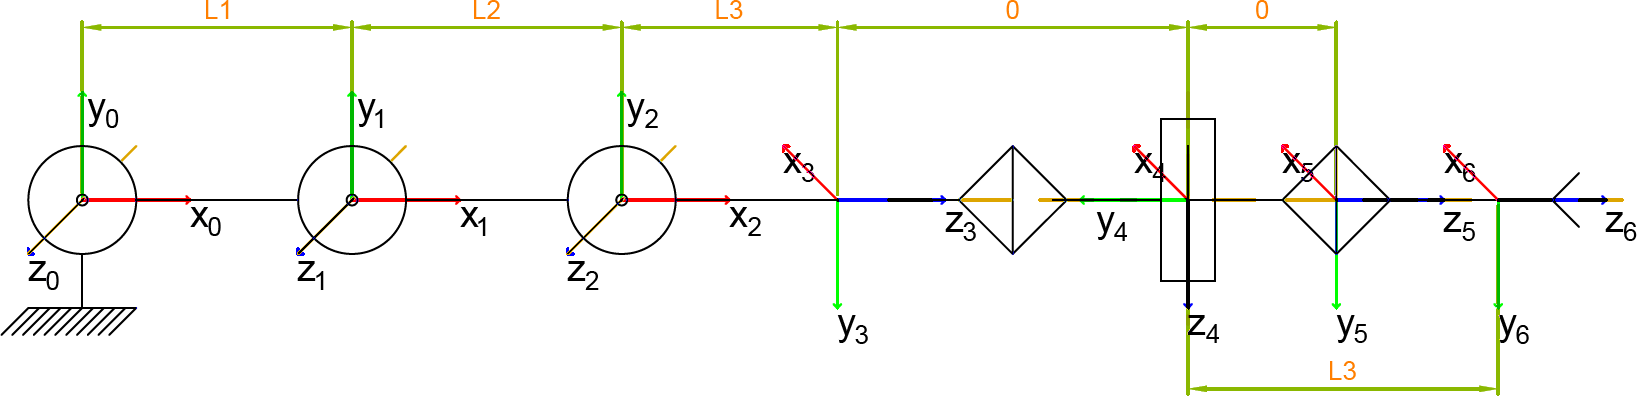
\includegraphics[width=\textwidth]{Strutture+Polso/RRRplanare+p.png}
\end{minipage}
\hfill
\begin{minipage}{0.5\textwidth}
\centering
\begin{tabular}{c|c|c|c|c|}  
            \cline{2-5} &
            \multicolumn{2}{|c|}{$A_z(\theta,d)$} &
            \multicolumn{2}{|c|}{$A_x(\alpha,a)$} \\
            \hline
        \multicolumn{1}{|c|}{$R_1$} & $q_{1}$ & $0$ & $0$ & $D_{1}$ \\
            \hline
        \multicolumn{1}{|c|}{$R_2$} & $q_{2}$ & $0$ & $0$ & $D_{2}$ \\
            \hline
        \multicolumn{1}{|c|}{$R_3$} & $q_{3}$ & $0$ & $0$ & $D_{3}$ \\
            \hline
\end{tabular}

\end{minipage}


\section*{Sferico 1 con Polso}
\begin{minipage}{0.5\textwidth}
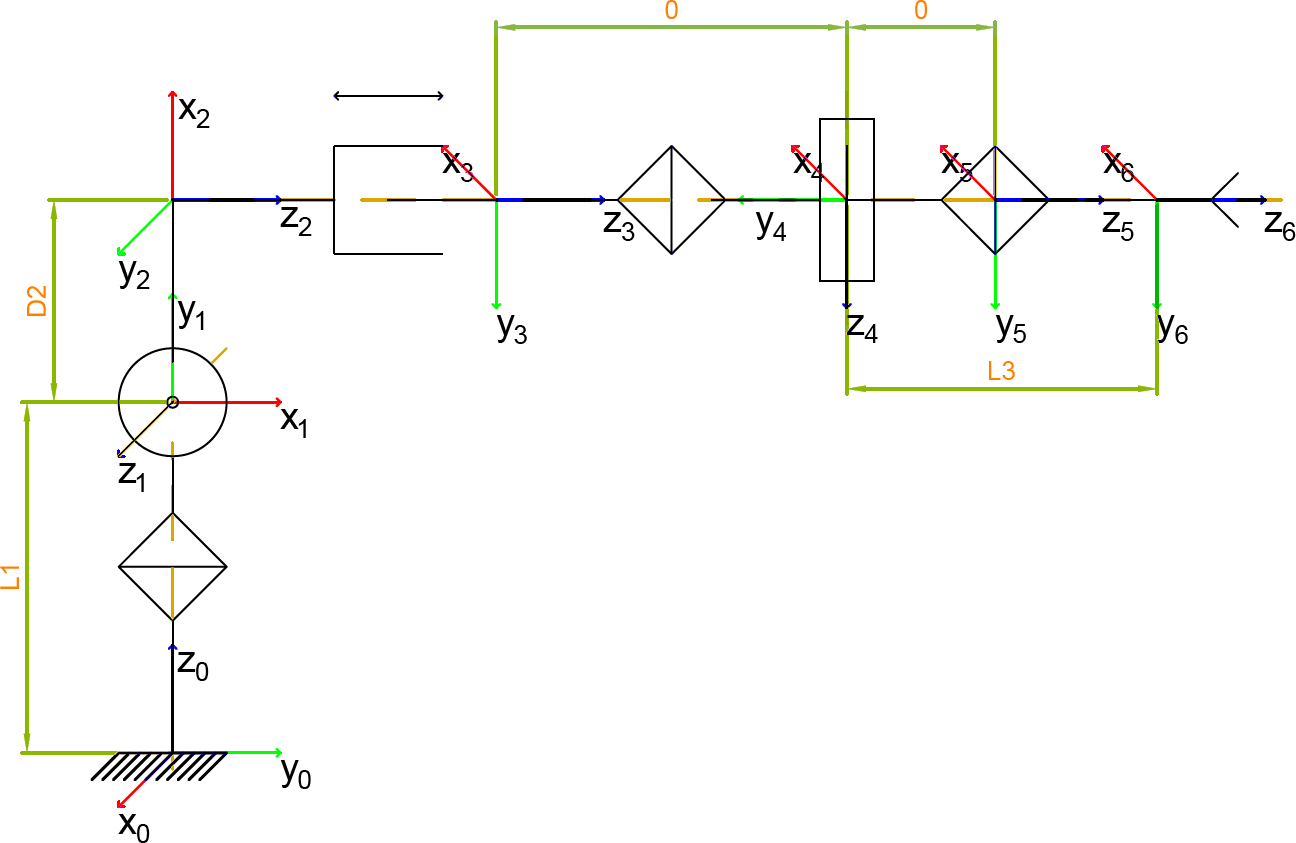
\includegraphics[width=\textwidth]{Strutture+Polso/Sferico1+p.png}
\end{minipage}
\hfill
\begin{minipage}{0.5\textwidth}
\centering
\begin{tabular}{c|c|c|c|c|}
            \cline{2-5} &
            \multicolumn{2}{|c|}{$A_z(\theta,d)$} &
            \multicolumn{2}{|c|}{$A_x(\alpha,a)$} \\
            \hline
        \multicolumn{1}{|c|}{$R_1$} & $q_{1}$ & $0$ & $0$ & $D_{1}$ \\
            \hline
        \multicolumn{1}{|c|}{$R_2$} & $q_{2}$ & $0$ & $0$ & $D_{2}$ \\
            \hline
        \multicolumn{1}{|c|}{$R_3$} & $q_{3}$ & $0$ & $0$ & $D_{3}$ \\
            \hline
\end{tabular}
$$\pmatrix{-\cos _{q_{1}}\,\cos _{q_{2}}\,\sin _{q_{4}}\,\sin _{q_{6}
 }+\sin _{q_{1}}\,\cos _{q_{4}}\,\sin _{q_{6}}-\cos _{q_{1}}\,\sin _{
 q_{2}}\,\sin _{q_{5}}\,\cos _{q_{6}}+\sin _{q_{1}}\,\sin _{q_{4}}\,
 \cos _{q_{5}}\,\cos _{q_{6}}+\cos _{q_{1}}\,\cos _{q_{2}}\,\cos _{
 q_{4}}\,\cos _{q_{5}}\,\cos _{q_{6}}&\cos _{q_{1}}\,\sin _{q_{2}}\,
 \sin _{q_{5}}\,\sin _{q_{6}}-\sin _{q_{1}}\,\sin _{q_{4}}\,\cos _{
 q_{5}}\,\sin _{q_{6}}-\cos _{q_{1}}\,\cos _{q_{2}}\,\cos _{q_{4}}\,
 \cos _{q_{5}}\,\sin _{q_{6}}-\cos _{q_{1}}\,\cos _{q_{2}}\,\sin _{
 q_{4}}\,\cos _{q_{6}}+\sin _{q_{1}}\,\cos _{q_{4}}\,\cos _{q_{6}}&
 \sin _{q_{1}}\,\sin _{q_{4}}\,\sin _{q_{5}}+\cos _{q_{1}}\,\cos _{
 q_{2}}\,\cos _{q_{4}}\,\sin _{q_{5}}+\cos _{q_{1}}\,\sin _{q_{2}}\,
 \cos _{q_{5}}&L_{6}\,\sin _{q_{1}}\,\sin _{q_{4}}\,\sin _{q_{5}}+
 L_{6}\,\cos _{q_{1}}\,\cos _{q_{2}}\,\cos _{q_{4}}\,\sin _{q_{5}}+
 L_{6}\,\cos _{q_{1}}\,\sin _{q_{2}}\,\cos _{q_{5}}+\cos _{q_{1}}\,
 \sin _{q_{2}}\,q_{3}+D_{2}\,\cos _{q_{1}}\,\cos _{q_{2}}\cr -\sin _{
 q_{1}}\,\cos _{q_{2}}\,\sin _{q_{4}}\,\sin _{q_{6}}-\cos _{q_{1}}\,
 \cos _{q_{4}}\,\sin _{q_{6}}-\sin _{q_{1}}\,\sin _{q_{2}}\,\sin _{
 q_{5}}\,\cos _{q_{6}}-\cos _{q_{1}}\,\sin _{q_{4}}\,\cos _{q_{5}}\,
 \cos _{q_{6}}+\sin _{q_{1}}\,\cos _{q_{2}}\,\cos _{q_{4}}\,\cos _{
 q_{5}}\,\cos _{q_{6}}&\sin _{q_{1}}\,\sin _{q_{2}}\,\sin _{q_{5}}\,
 \sin _{q_{6}}+\cos _{q_{1}}\,\sin _{q_{4}}\,\cos _{q_{5}}\,\sin _{
 q_{6}}-\sin _{q_{1}}\,\cos _{q_{2}}\,\cos _{q_{4}}\,\cos _{q_{5}}\,
 \sin _{q_{6}}-\sin _{q_{1}}\,\cos _{q_{2}}\,\sin _{q_{4}}\,\cos _{
 q_{6}}-\cos _{q_{1}}\,\cos _{q_{4}}\,\cos _{q_{6}}&-\cos _{q_{1}}\,
 \sin _{q_{4}}\,\sin _{q_{5}}+\sin _{q_{1}}\,\cos _{q_{2}}\,\cos _{
 q_{4}}\,\sin _{q_{5}}+\sin _{q_{1}}\,\sin _{q_{2}}\,\cos _{q_{5}}&-
 L_{6}\,\cos _{q_{1}}\,\sin _{q_{4}}\,\sin _{q_{5}}+L_{6}\,\sin _{
 q_{1}}\,\cos _{q_{2}}\,\cos _{q_{4}}\,\sin _{q_{5}}+L_{6}\,\sin _{
 q_{1}}\,\sin _{q_{2}}\,\cos _{q_{5}}+\sin _{q_{1}}\,\sin _{q_{2}}\,
 q_{3}+D_{2}\,\sin _{q_{1}}\,\cos _{q_{2}}\cr -\sin _{q_{2}}\,\sin _{
 q_{4}}\,\sin _{q_{6}}+\cos _{q_{2}}\,\sin _{q_{5}}\,\cos _{q_{6}}+
 \sin _{q_{2}}\,\cos _{q_{4}}\,\cos _{q_{5}}\,\cos _{q_{6}}&-\cos _{
 q_{2}}\,\sin _{q_{5}}\,\sin _{q_{6}}-\sin _{q_{2}}\,\cos _{q_{4}}\,
 \cos _{q_{5}}\,\sin _{q_{6}}-\sin _{q_{2}}\,\sin _{q_{4}}\,\cos _{
 q_{6}}&\sin _{q_{2}}\,\cos _{q_{4}}\,\sin _{q_{5}}-\cos _{q_{2}}\,
 \cos _{q_{5}}&L_{6}\,\sin _{q_{2}}\,\cos _{q_{4}}\,\sin _{q_{5}}-
 L_{6}\,\cos _{q_{2}}\,\cos _{q_{5}}-\cos _{q_{2}}\,q_{3}+D_{2}\,
 \sin _{q_{2}}+L_{1}\cr 0&0&0&1\cr }$$

\end{minipage}


\section*{Sferico di Stanford con Polso}
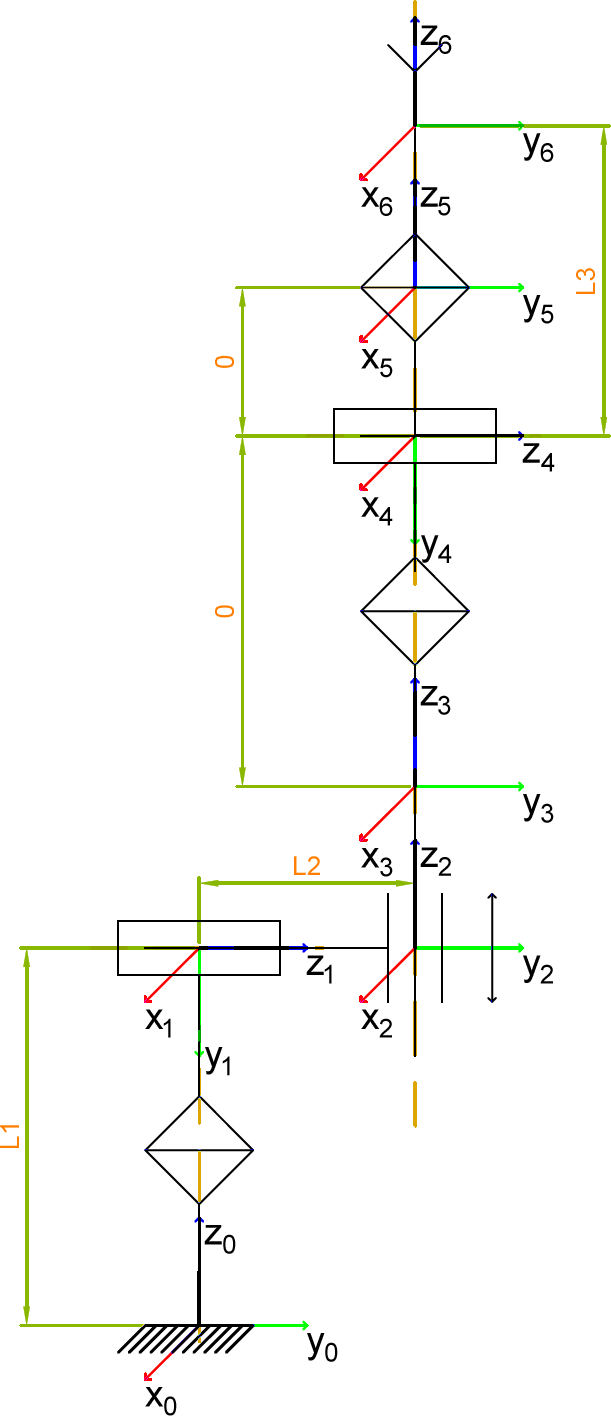
\includegraphics[height=0.5\textheight]{Strutture+Polso/SfericoStanford+p.png}
\centering{\tiny{\begin{tabular}{c|c|c|c|c|}
            \cline{2-5} &
            \multicolumn{2}{|c|}{$A_z(\theta,d)$} &
            \multicolumn{2}{|c|}{$A_x(\alpha,a)$} \\
            \hline
        \multicolumn{1}{|c|}{$R_1$} & $q_{1}$ & $0$ & $0$ & $D_{1}$ \\
            \hline
        \multicolumn{1}{|c|}{$R_2$} & $q_{2}$ & $0$ & $0$ & $D_{2}$ \\
            \hline
        \multicolumn{1}{|c|}{$R_3$} & $q_{3}$ & $0$ & $0$ & $D_{3}$ \\
            \hline
\end{tabular}
}}



\section*{Antropomorfo con Polso}
\begin{minipage}{0.5\textwidth}
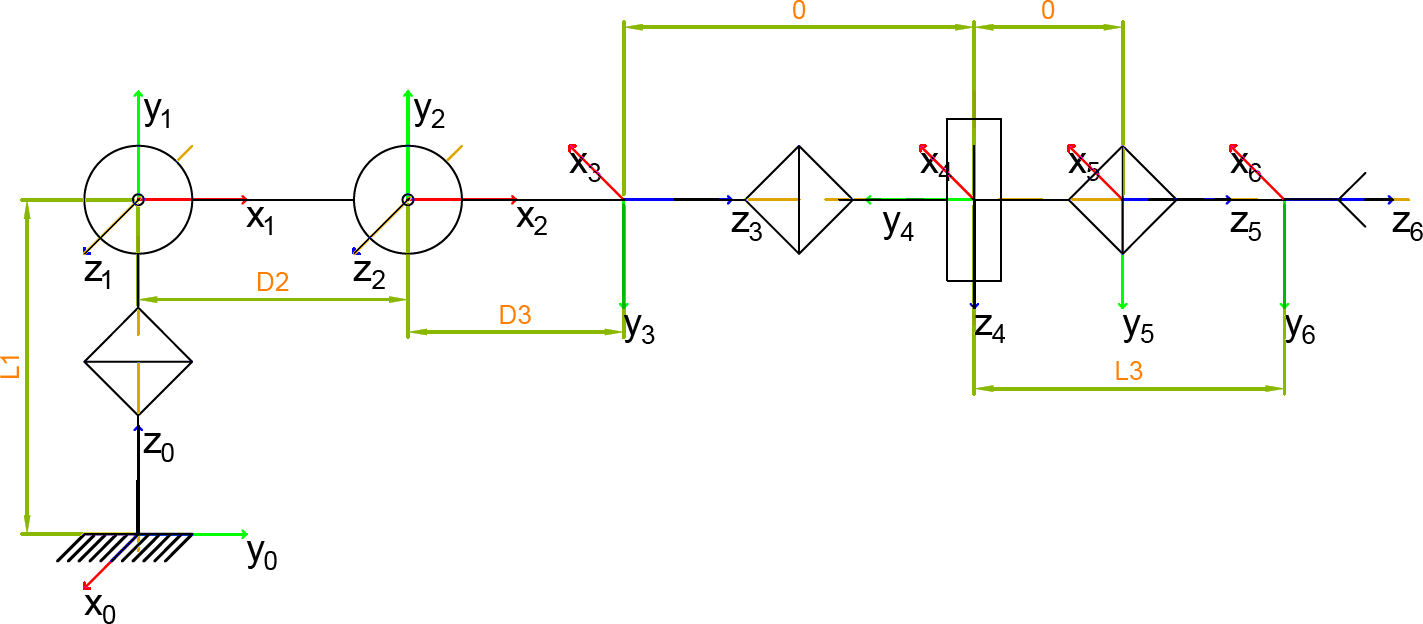
\includegraphics[width=\textwidth]{Strutture+Polso/Antropomorfo+p.png}
\end{minipage}
\hfill
\begin{minipage}{0.5\textwidth}
\centering
\begin{tabular}{c|c|c|c|c|}
            \cline{2-5} &
            \multicolumn{2}{|c|}{$A_z(\theta,d)$} &
            \multicolumn{2}{|c|}{$A_x(\alpha,a)$} \\
            \hline
        \multicolumn{1}{|c|}{$R_1$} & $q_{1}$ & $0$ & $0$ & $D_{1}$ \\
            \hline
        \multicolumn{1}{|c|}{$R_2$} & $q_{2}$ & $0$ & $0$ & $D_{2}$ \\
            \hline
        \multicolumn{1}{|c|}{$R_3$} & $q_{3}$ & $0$ & $0$ & $D_{3}$ \\
            \hline
\end{tabular}

\end{minipage}


\end{document}